\section{Reach Set Estimation}\label{s:ReachSetEstimationTheory}
\paragraph{Idea:} The basic idea for \emph{Discrete Reach set Estimation  method} is taken from \cite{ljungqvist2017lattice}. The focus of their work is to generate paths that are kinematically feasible. Path following controllers in order to find techniques to stabilize the system around these paths \cite{ljungqvist2016path,evestedt2016path}. 

Lattice-based planners have been deployed with great success on several robotic platforms \cite{pivtoraiko2009differentially,urmson2008william,cirillo2017videogames,tomlin2000game,chen1997game}. However, a problem with lattice-based approaches is the exponential complexity in the dimension of the state space which can limit the use for more complicated models.

The optimization problem was solved real-time by \emph{Avocado solver} \cite{houska2011acado}.

\paragraph{Example:} The \emph{example of movement lattice} is given in (fig. \ref{fig:latticeMovementPrimitivesExample}). Truck (black rectangle) is towing Trailer (red rectangle). The \emph{state} has only one \emph{reach set impacting variable} - \emph{trailer displacement}. When trailer displacement is $0^{\circ}$ (fig. \ref{fig:noDisplacementLattuce}) the lattice representation of \emph{Reach Set} is different that in case of small left/right tilt (fig. \ref{fig:displacementleftrightlattuce}).

\begin{figure}[H]
    \centering
    \begin{subfigure}{0.48\textwidth}
        \centering
        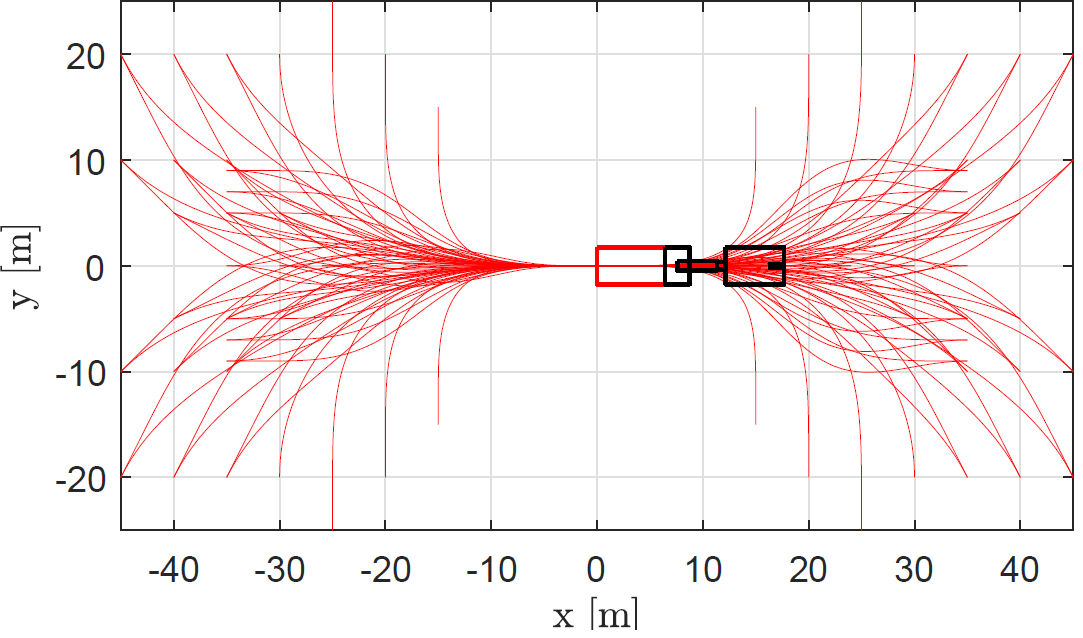
\includegraphics[width=0.9\linewidth]{\FIGDIR/TE028LattuceMovementSet01}
        \caption{Trailer displacement $0^{\circ}$.}
        \label{fig:noDisplacementLattuce}
    \end{subfigure}
    \begin{subfigure}{0.48\textwidth}
        \centering
        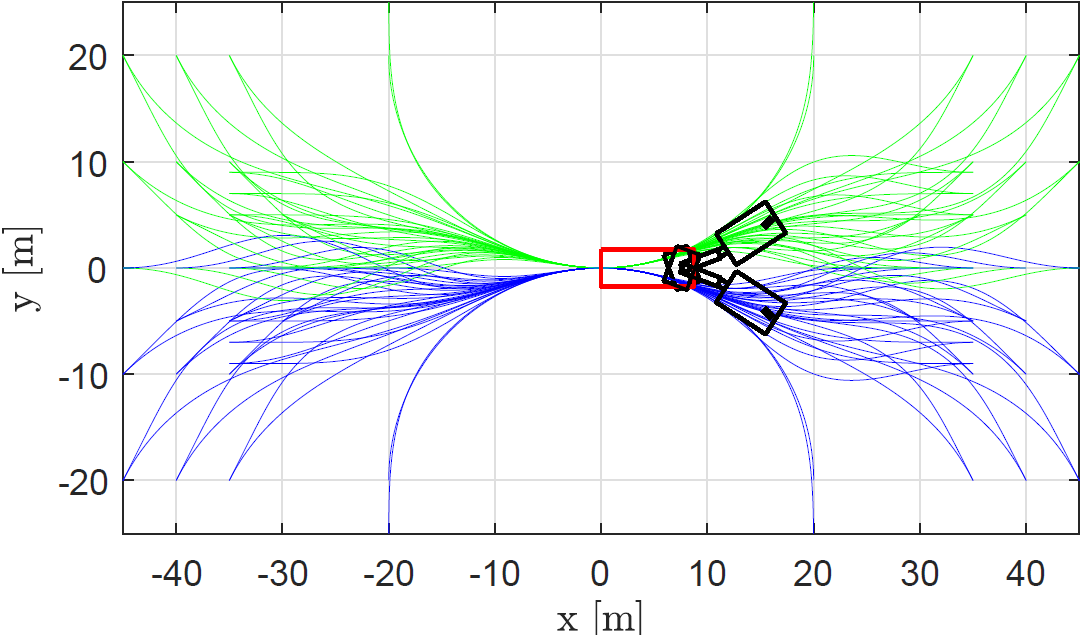
\includegraphics[width=0.9\linewidth]{\FIGDIR/TE029LattuceMovementSe02t} 
        \caption{$12^{\circ}$ (green) $-12^{\circ}$ (blue).}
        \label{fig:displacementleftrightlattuce}
    \end{subfigure}
    
    \caption{\emph{Movement set primitives} for Lattice-Based Movement Planning. \cite{ljungqvist2017lattice}. }
    \label{fig:latticeMovementPrimitivesExample}
\end{figure}

\paragraph{Benefits:} Presented method of \emph{Lattice Search}  is  de-facto \emph{Reduced Reach Set Approximation} in open space for \emph{Truck-Trailer} system. 

The idea of \emph{Movement primitives} is very close to \emph{Movement Automaton} (def. \ref{def:movementAutomaton}), which can be used as a \emph{control interface} effectively. 

The \emph{Constraints} of obstacle set in \emph{Known world} (sec. \ref{s:KnownWorld}) are supported to some degree.

\paragraph{Shortcomings:} The lattice search approach has the following shortcoming:
\begin{enumerate}
    \item \emph{Limited system dimension} - given method works in \emph{real time} only if dimension of \emph{system state space} does not exceed $4^{th}$  rank.
    
    \item \emph{Real-time optimization} - real-time optimization is main cause of \emph{limited system dimension}. If the decision time can be discrete (which movement automaton enforces), then offline optimization  can be used. 
    
    \item \emph{Continuous space disparity} - the example (fig. \ref{fig:latticeMovementPrimitivesExample}) shows there are member variables of \emph{State Space} which significantly impacts the shape of the lattice (reach set estimation). Space disparity  is not a problem in real-time environment. The discretization of \emph{time-domain} raises this as a shortcoming.
    
    \item \emph{Trajectory Tracking} - approach generates \emph{Continuous Domain} reference signal. For \emph{Discrete Domain}, it is necessary to address this issue.
\end{enumerate}

 




